\subsection{Source data}
The data come from the Kaggle competition \emph{Walmart Recruiting -- Store Sales Forecasting}~\cite{kaggle_walmart} and consist of three related tables. The \texttt{train} table holds 421{,}570 department-week records (\texttt{Store}, \texttt{Dept}, \texttt{Date}, \texttt{Weekly\_Sales}, \texttt{IsHoliday}) for 45 stores and 81 departments, from 5~February~2010 to 26~October~2012. The \texttt{features} table adds, for every store-week, the average regional \texttt{Temperature}, the regional \texttt{Fuel\_Price}, five anonymised promotional variables \texttt{MarkDown1}--\texttt{MarkDown5}, the \texttt{CPI} and the regional \texttt{Unemployment} rate. The \texttt{stores} table gives each store's \texttt{Type} (A, B or C) and floor \texttt{Size}. The three tables are joined on (\texttt{Store}, \texttt{Date}) and \texttt{Store}, respectively. The four holiday weeks flagged by Walmart --- Super Bowl, Labor Day, Thanksgiving and Christmas --- are known to be weighted five times more heavily in the original competition metric.

\subsection{Noise audit}
The cover specification of this project asks for a ``difficult dataset with noise''. Table~\ref{tab:noise} quantifies why the Walmart data qualify. The target is extremely right-skewed (skewness 3.26; mean \$15{,}981 versus median \$7{,}612; maximum \$693{,}099). 1{,}285 records have \emph{negative} sales (net returns), and 35{,}521 records (8.4\%) lie outside the $1.5\times$IQR whiskers. The promotional variables are missing for 64--74\% of the rows, mostly because MarkDowns were only recorded from November 2011 onward, and 1{,}568 MarkDown values are negative, which is impossible for a discount amount and must be treated as entry errors. Finally, the store-week context variables (temperature, fuel price, CPI, unemployment) are measured at the store or region level and are therefore identical for all $\approx$74 departments of a store in a given week: for the department-level target they act as weak, highly redundant covariates.

\begin{table}[!t]
\caption{Noise and quality issues in the merged dataset (421{,}570 rows)}
\label{tab:noise}
\centering
\begin{tabular}{lrr}
\toprule
Issue & Count & \% rows \\
\midrule
Negative weekly sales (returns) & 1{,}285 & 0.30 \\
Weekly-sales outliers ($1.5\times$IQR) & 35{,}521 & 8.43 \\
MarkDown1 missing & 270{,}889 & 64.26 \\
MarkDown2 missing & 310{,}322 & 73.61 \\
MarkDown3 missing & 284{,}479 & 67.48 \\
MarkDown4 missing & 286{,}603 & 67.98 \\
MarkDown5 missing & 270{,}138 & 64.08 \\
Negative MarkDown values & 1{,}568 & 0.37 \\
Holiday-week rows & 29{,}661 & 7.04 \\
Skewness of \texttt{Weekly\_Sales} & \multicolumn{2}{c}{3.26} \\
\bottomrule
\end{tabular}
\end{table}

\subsection{Target definition}
We define three ordered classes by the 33.3th and 66.7th percentiles of \texttt{Weekly\_Sales}: \textbf{Low} ($\le\$3{,}521.78$), \textbf{Medium} ($\$3{,}521.78$--$\$14{,}599.76$) and \textbf{High} ($>\$14{,}599.76$). By construction the classes are balanced (140{,}524 / 140{,}523 / 140{,}523 rows), so accuracy is a meaningful headline metric and the chance level is 33.3\%. Negative sales are kept --- they are genuine business events --- and fall into the Low class.

\subsection{Preprocessing}
\begin{enumerate}
\item \textbf{Missing promotions.} A missing MarkDown means that no promotion was recorded, so it is replaced by zero, and a binary \texttt{MarkDown\_Available} flag preserves the information that the value was missing.
\item \textbf{Promotion noise.} Negative MarkDowns are clipped to zero, and each MarkDown is winsorised at its 99.5th percentile to limit the leverage of extreme promotions.
\item \textbf{Calendar features.} From \texttt{Date} we derive \texttt{Year}, \texttt{Month}, ISO \texttt{Week} and \texttt{Day}; the signed number of days to Thanksgiving and to Christmas of the same year; and binary Super Bowl and Labor Day indicators.
\item \textbf{Encoding.} Store \texttt{Type} is one-hot encoded (\texttt{Type\_A}, \texttt{Type\_B}, \texttt{Type\_C}) and \texttt{IsHoliday} is cast to an integer.
\end{enumerate}
The final design matrix has \textbf{25 features}, listed in Table~\ref{tab:features}, and no missing values.

\begin{table}[!t]
\caption{The 25 model features}
\label{tab:features}
\centering
\begin{tabular}{p{1.9cm}p{5.9cm}}
\toprule
Group & Features \\
\midrule
Identity & Store, Dept \\
Store & Size, Type\_A, Type\_B, Type\_C \\
Economy & Temperature, Fuel\_Price, CPI, Unemployment \\
Promotion & MarkDown1--5, MarkDown\_Available \\
Calendar & IsHoliday, Year, Month, Week, Day, Days\_to\_Thanksgiving, Days\_to\_Christmas, SuperBowl, LaborDay \\
\bottomrule
\end{tabular}
\end{table}

\subsection{Exploratory analysis}
Fig.~\ref{fig:eda} summarises the data before any reduction. Total chain-wide sales are flat for most of the year and spike sharply in the flagged Thanksgiving week (about \$66M versus a typical \$45--50M) and in the week \emph{before} Christmas (up to \$81M). The flagged Christmas week itself, which ends on the last Friday of December, is actually a dip, and the Super Bowl and Labor Day weeks show no visible spike. Only one of the four official holiday weeks therefore coincides with a peak, which already hints that the \texttt{IsHoliday} flag is a weak predictor. Store size increases from Type C to Type A stores; within Types A and B the High class is associated with larger stores, whereas Type C stores all have almost the same size. Fig.~\ref{fig:corr} shows the Spearman correlation matrix: the strongest monotone association with the sales class is \texttt{Size} ($\rho=0.26$), followed by the store-type dummies ($|\rho|=0.10$--$0.19$); all other features have $|\rho|<0.08$. In particular, \texttt{Dept} has an almost zero rank correlation with the class ($\rho=-0.03$) even though, as shown later, it is by far the most informative variable: its effect is strong but entirely \emph{non-monotone}, because department numbers are arbitrary identifiers. The calendar variables \texttt{Week}, \texttt{Month}, \texttt{Days\_to\_Thanksgiving} and \texttt{Days\_to\_Christmas} are almost perfectly collinear, and so are the five MarkDowns, which indicates substantial redundancy for the reduction and selection methods to exploit.

\begin{figure*}[!t]
\centering
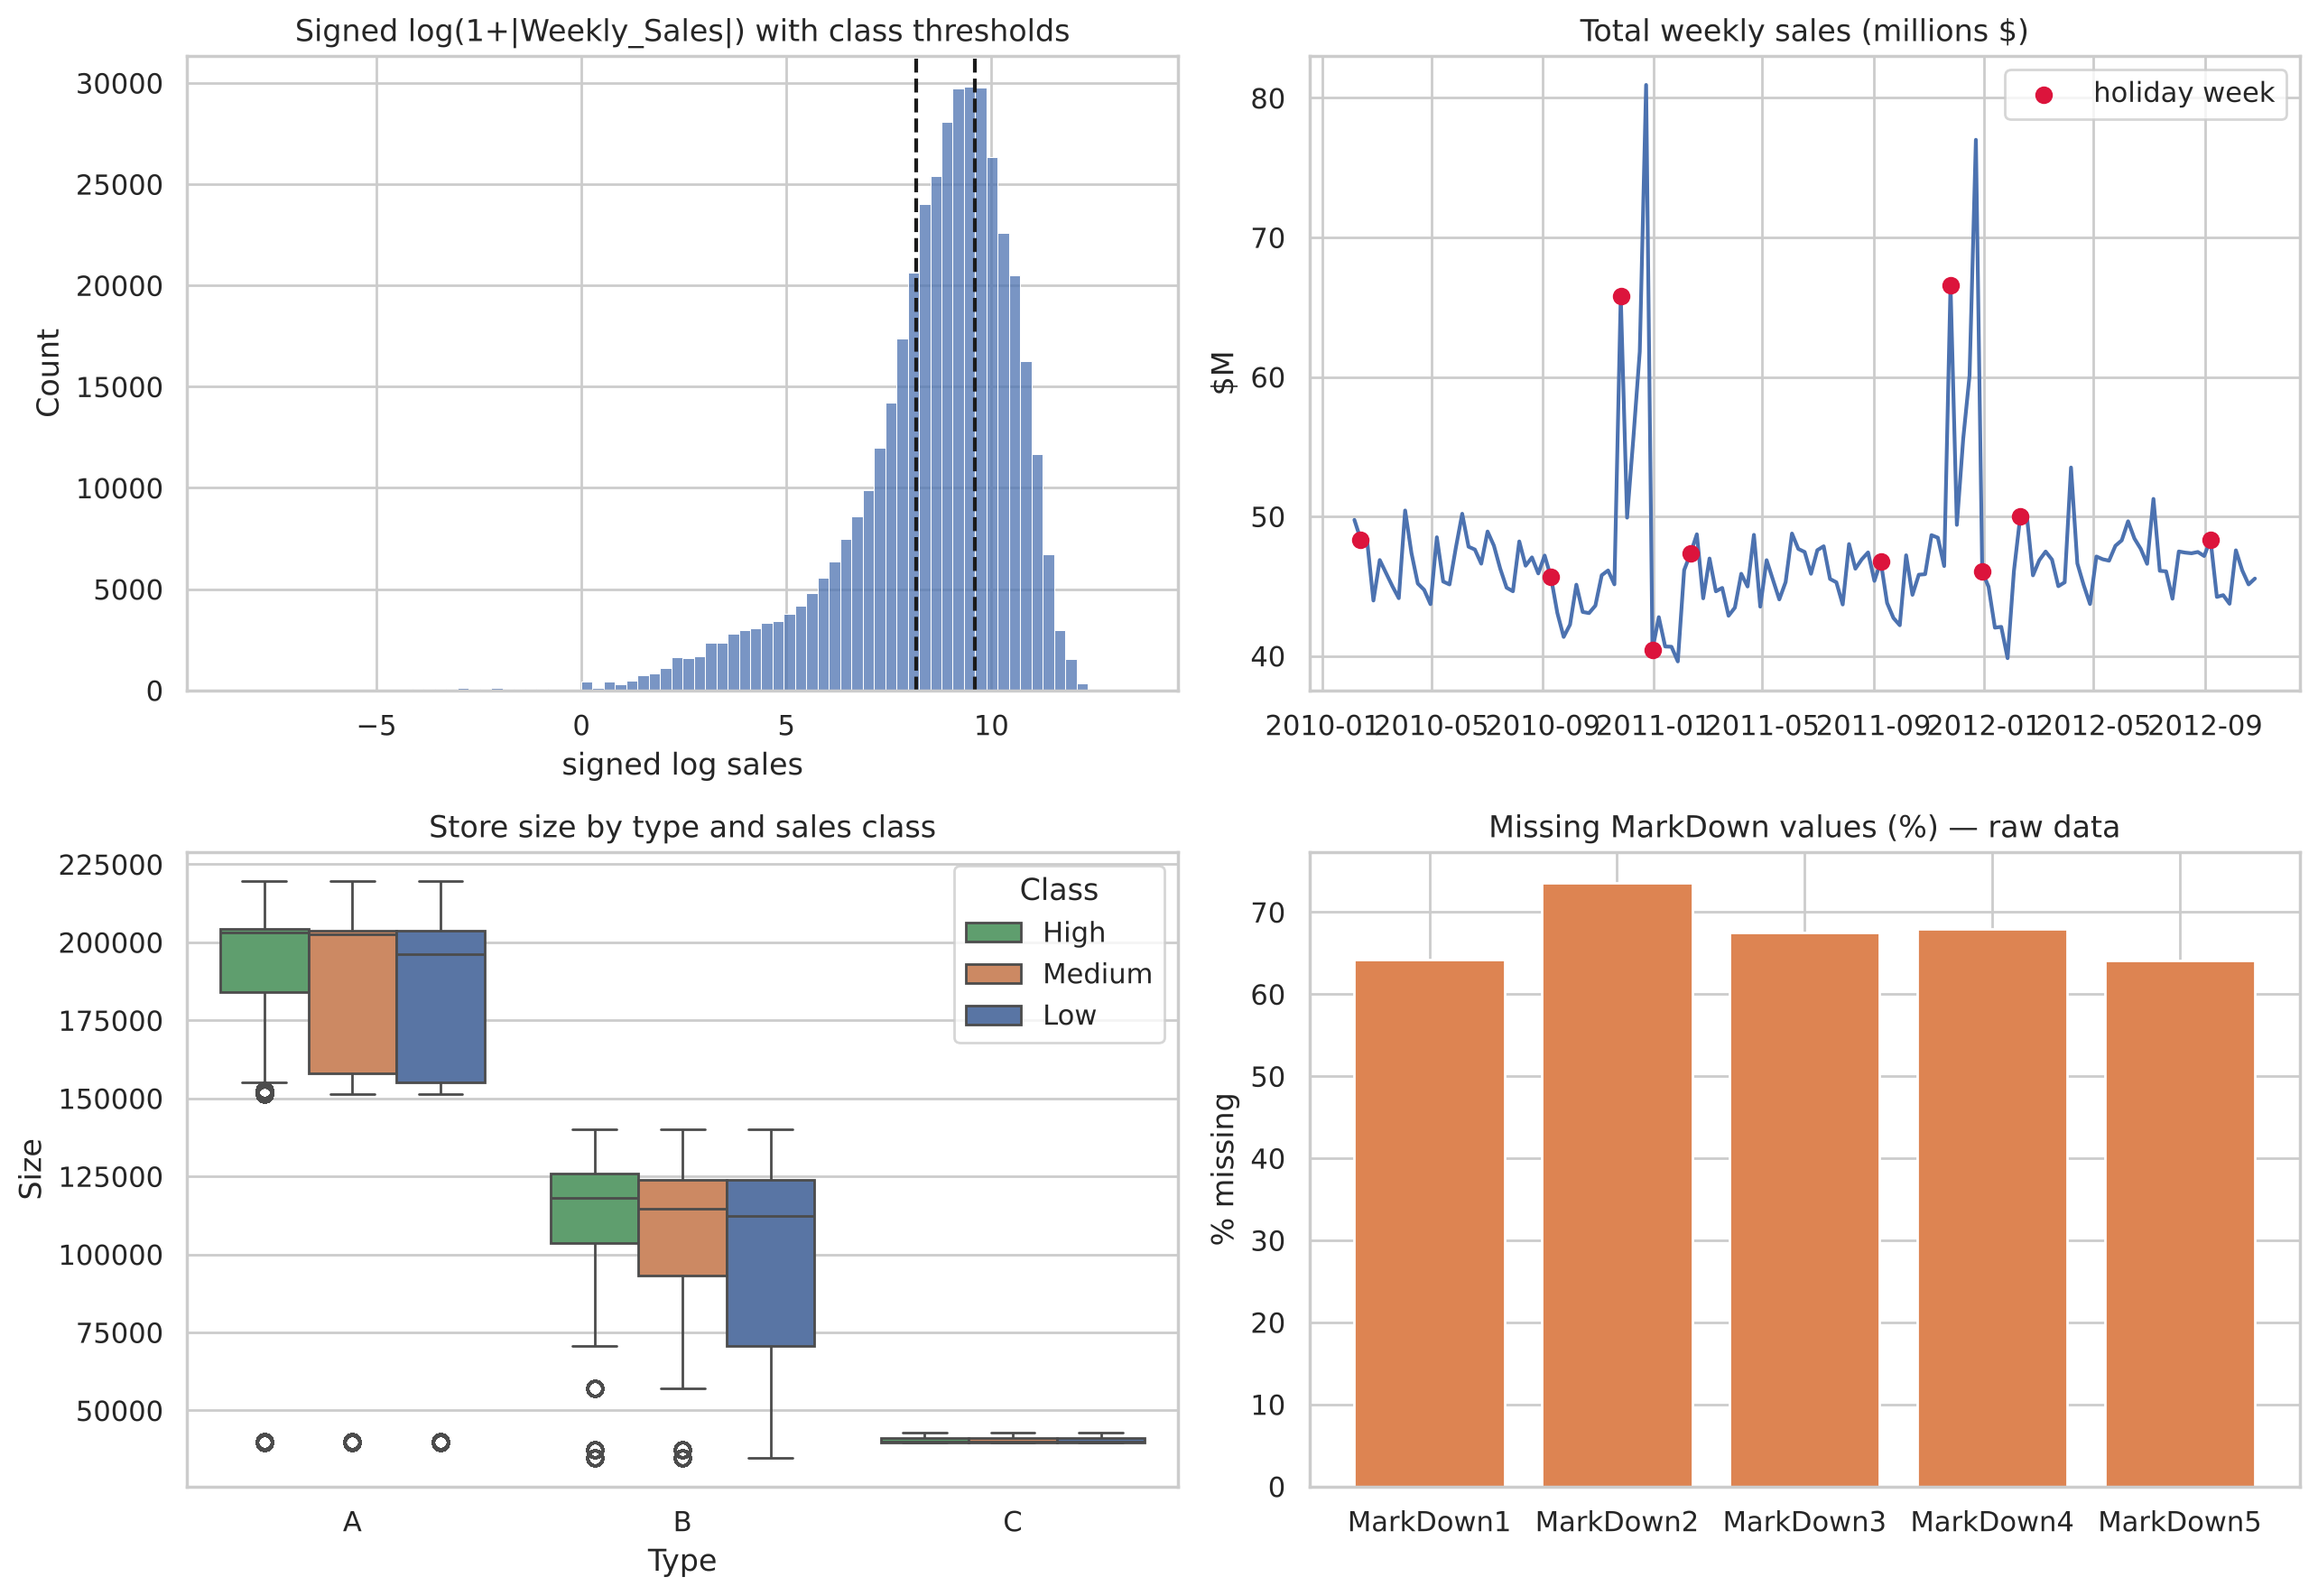
\includegraphics[width=0.86\textwidth]{figures/01_eda_overview.png}
\caption{Exploratory analysis before reduction. Top-left: signed $\log(1+|\text{sales}|)$ with the two class thresholds (dashed). Top-right: chain-wide weekly sales with holiday weeks in red. Bottom-left: store size by type and class. Bottom-right: share of missing MarkDown values in the raw data.}
\label{fig:eda}
\end{figure*}

\begin{figure}[!t]
\centering
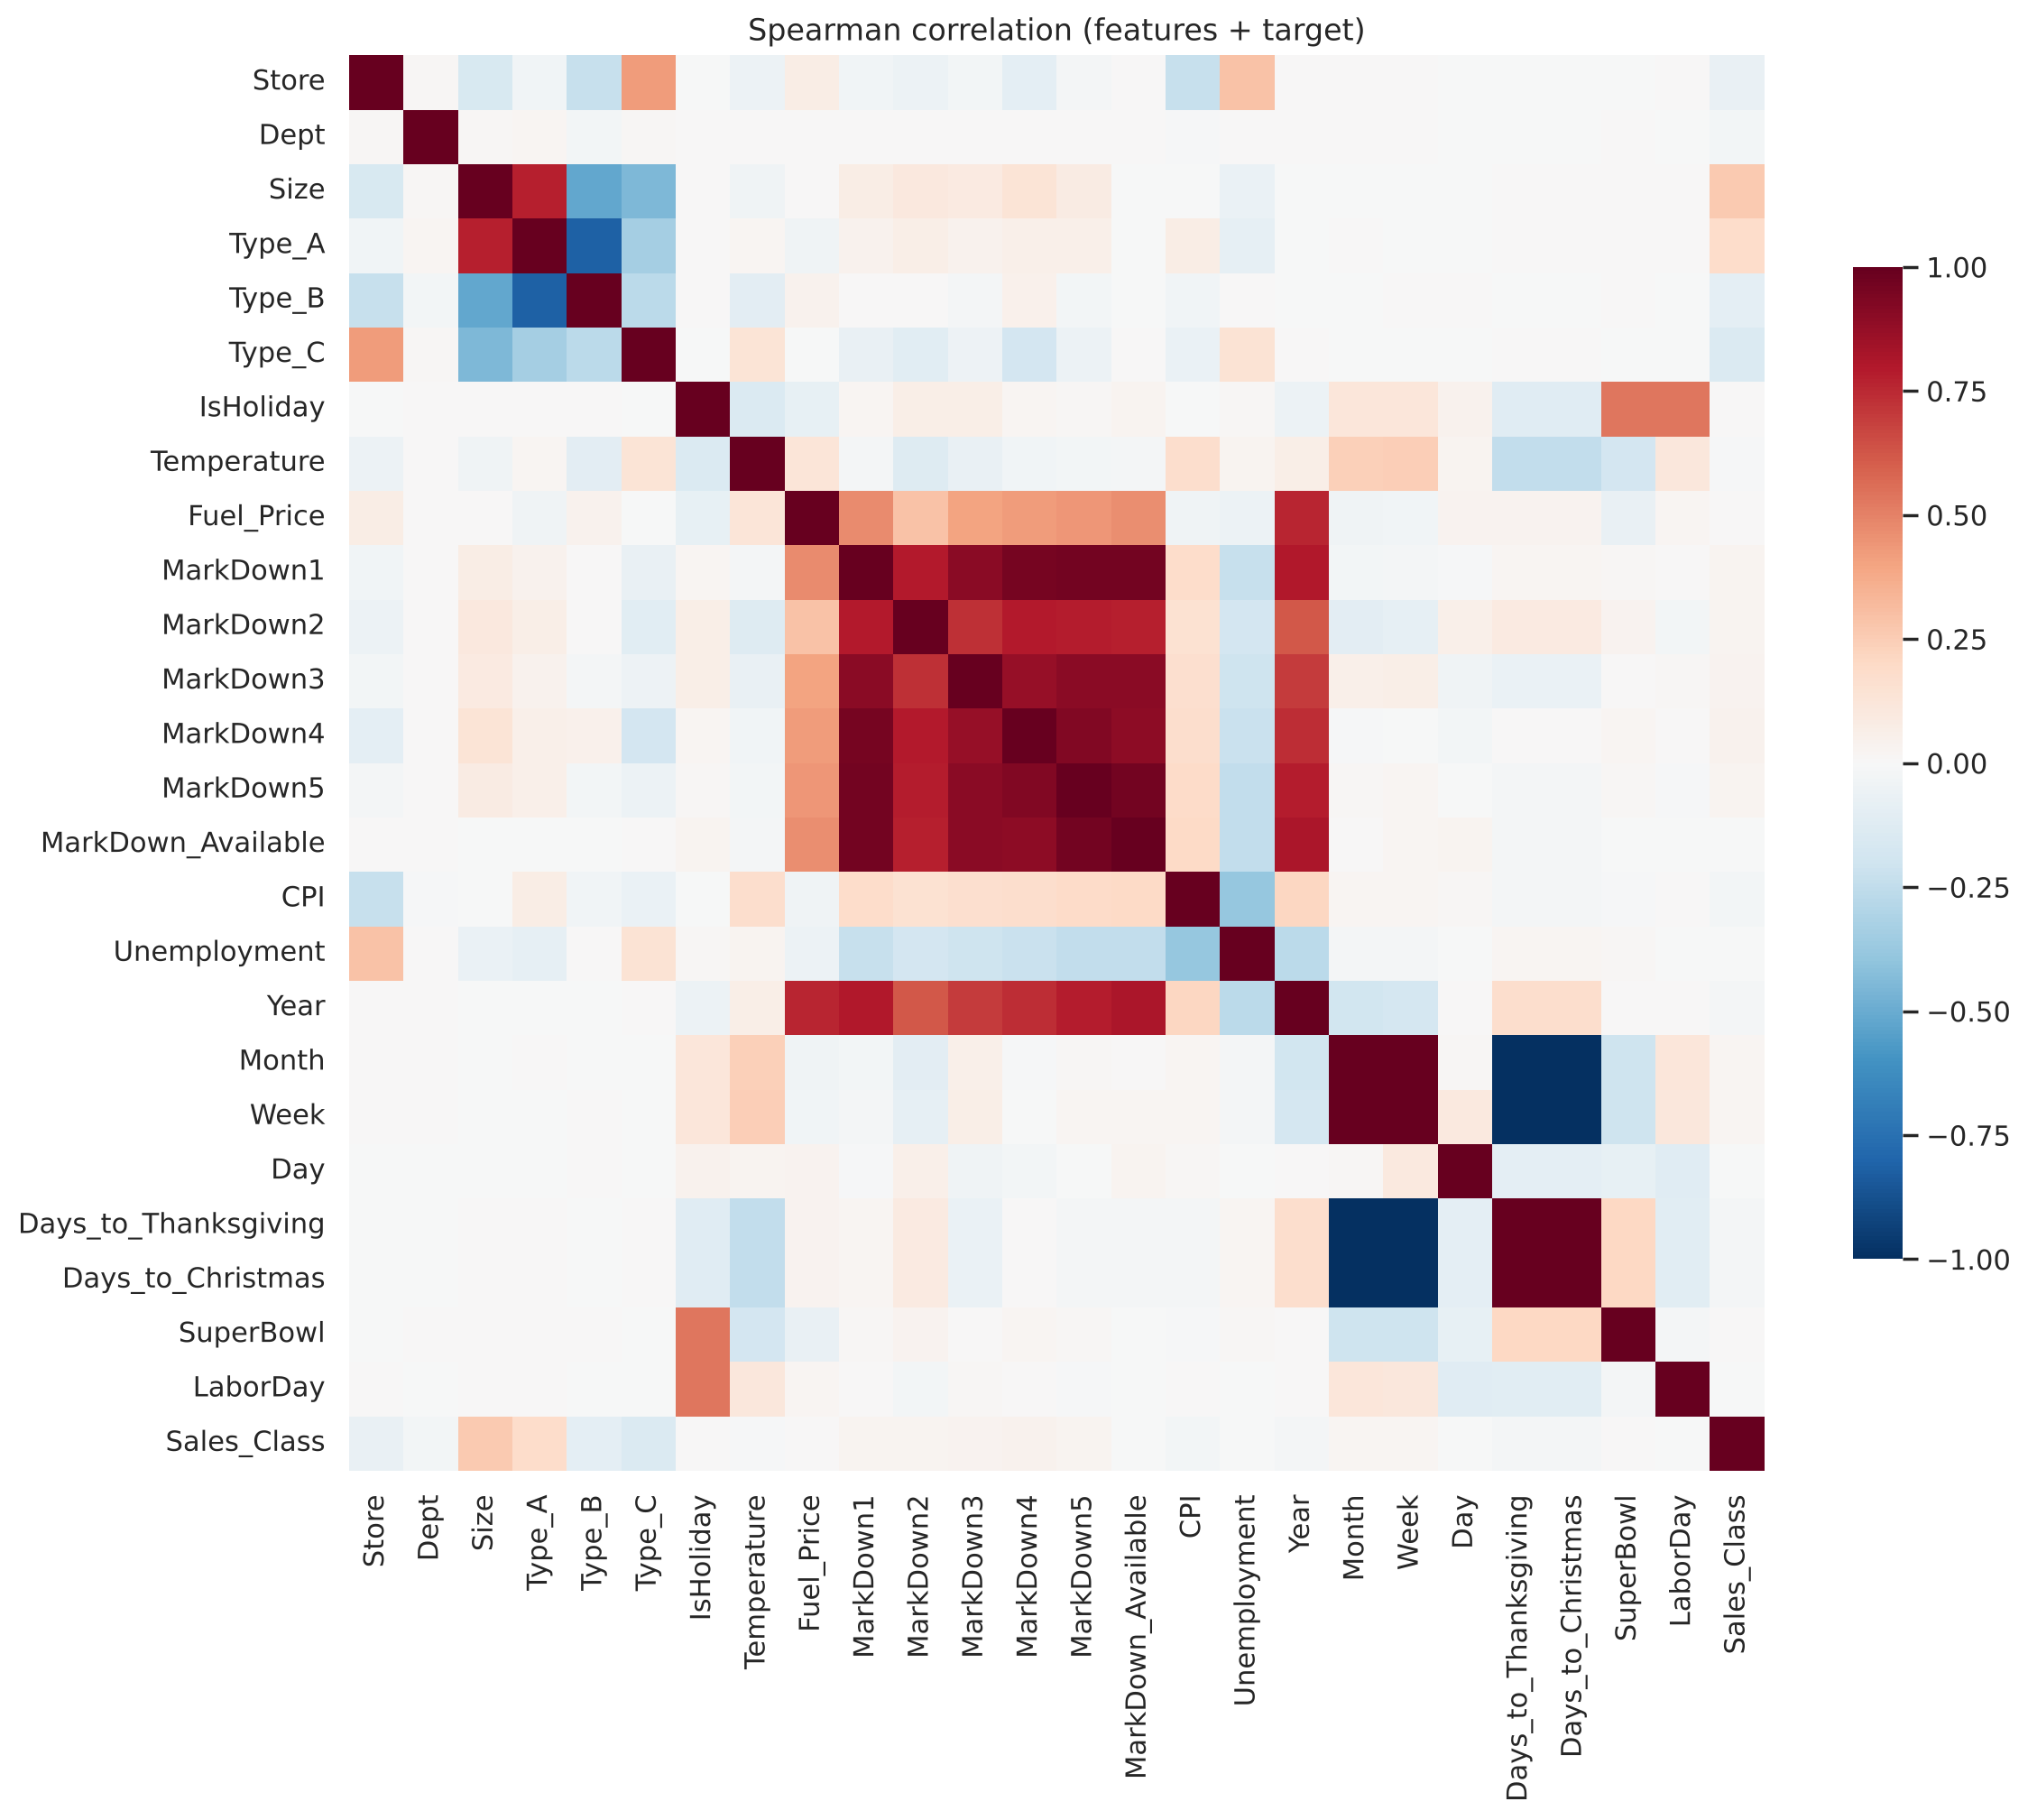
\includegraphics[width=\columnwidth]{figures/02_correlation.png}
\caption{Spearman correlation between the 25 features and the ordinal sales class (last row/column).}
\label{fig:corr}
\end{figure}

\subsection{Sampling and splitting}
Training nine models with 5-fold cross-validation, and running three metaheuristics that each evaluate several hundred feature subsets, on 421{,}570 rows is beyond the two-core, 8-GB machine used for this study. We therefore draw a \textbf{stratified sample of 100{,}000 rows} (23.7\% of the data) and split it \textbf{80/20} with stratification into 80{,}000 training and 20{,}000 test rows. Feature selection uses a 20{,}000-row subsample of the training split only, so the test rows never influence which features are chosen. The manifold methods, whose cost grows quadratically or cubically with $n$, use a 3{,}000-point subsample of the training split (1{,}500 points for SNE and 1{,}000 for MDS).
